%%
% The BIThesis Template for Bachelor Graduation Thesis
%
% 北京理工大学毕业设计(论文)第一章节 —— 使用 XeLaTeX 编译
%
% Copyright 2020 Spencer Woo
%
% This work may be distributed and/or modified under the
% conditions of the LaTeX Project Public License, either version 1.3
% of this license or (at your option) any later version.
% The latest version of this license is in
%   http://www.latex-project.org/lppl.txt
% and version 1.3 or later is part of all distributions of LaTeX
% version 2005/12/01 or later.
%
% This work has the LPPL maintenance status `maintained'.
%
% The Current Maintainer of this work is Spencer Woo.
%
% 第一章节

\chapter{黑洞可视化}

\section{程序设定}
\paragraph{坐标系}
之前的史瓦西测地线的推导是建立在四维球坐标系$\left(t,r,\theta,\phi\right)$上。本程序不考虑时间膨胀,将坐标系简化为$\left(r,\theta,\phi\right)$。三维图形的绘制是建立在笛卡尔坐标系$\left(x,y,z\right)$上。两者具有如下关系:
\begin{equation}
    \begin{split}
        x&=r\cos\theta\sin\phi\\
        y&=r\sin\theta\sin\phi\\
        z&=r\cos\theta
    \end{split}
\end{equation}
\paragraph{黑洞}程序中实现了一个不旋转不带电荷的史瓦西黑洞。黑洞奇点放置在世界坐标的原点$\left(0,0,0\right)$。史瓦西黑洞只具有一个性质:质量。黑洞的其他特征包括爱因斯坦环都由中心天体的质量决定。
\paragraph{吸积盘}吸积盘是一个类似土星环的黑洞拥有一个可选的圆形吸积盘。黑洞的吸积盘形态基本不取决于黑洞的质量,但会有一些物理上的限制。吸积盘固定于黑洞位于世界坐标系中的赤道面上。宇宙中没有绝对的方向,调整相机的视角和天空盒的坐标就可以控制吸积盘的倾角。
\paragraph{天空盒}
天空盒是一个正立方体,使用六张正方形图片描述从无限远处传来的光线。在这个程序中我使用右手定则来确定天空盒的坐标,与世界坐标系一致。天空盒的采样使用从世界原点出发的位置向量确定。使用像素天空盒,而不直接使用星表确定背景星空,是因为恒星与星系不是光线追踪的最小单位,光线才是。下图\ref{sub@fig:nasa-apod}\cite{raytraceusingstarcatalogue}是NASA每日一图(APOD)使用Star Catalogue生成的黑洞示意图,注意背景恒星是圆形的,爱因斯坦环确实弧形的。而真正所应看到的影像应该是类似\ref{sub@fig:nasa-apod-erratum},星光越接近黑洞视界越扭曲\footnote{我没有原始的完整的六面天空盒,红色部分是来自正面以外天空盒的光线}。
\begin{figure}[htbp]
    \centering
    \begin{subfigure}{.5\textwidth}
        \centering
        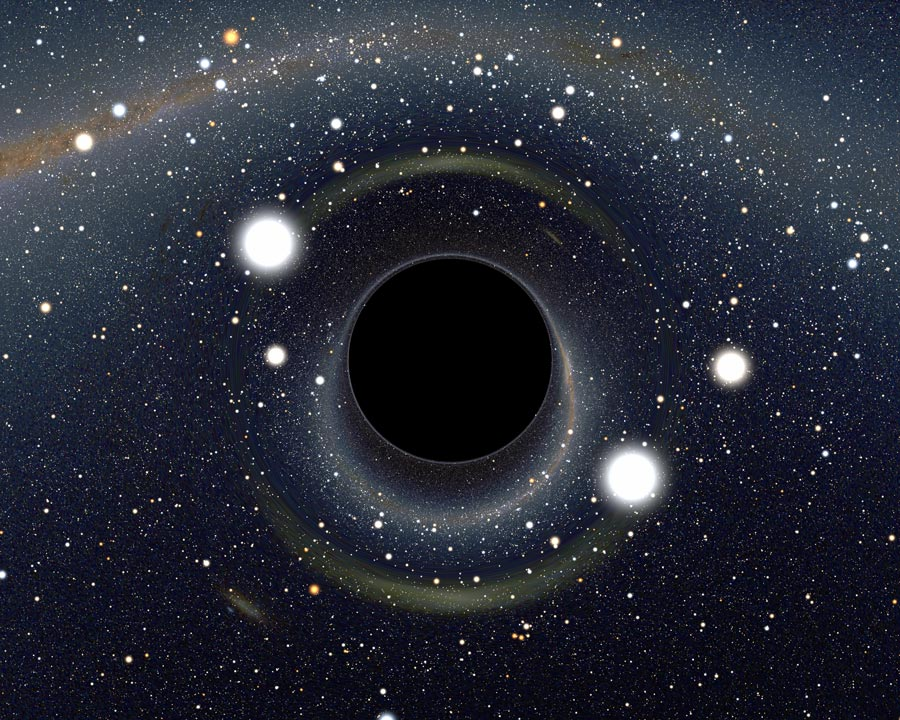
\includegraphics[width=.8\linewidth]{images/bhlens_riazuelo.jpg}
        \caption{NASA APOD 使用Star Catalogue生成的背景}
        \label{fig:nasa-apod}
    \end{subfigure}%
    \begin{subfigure}{.5\textwidth}
        \centering
        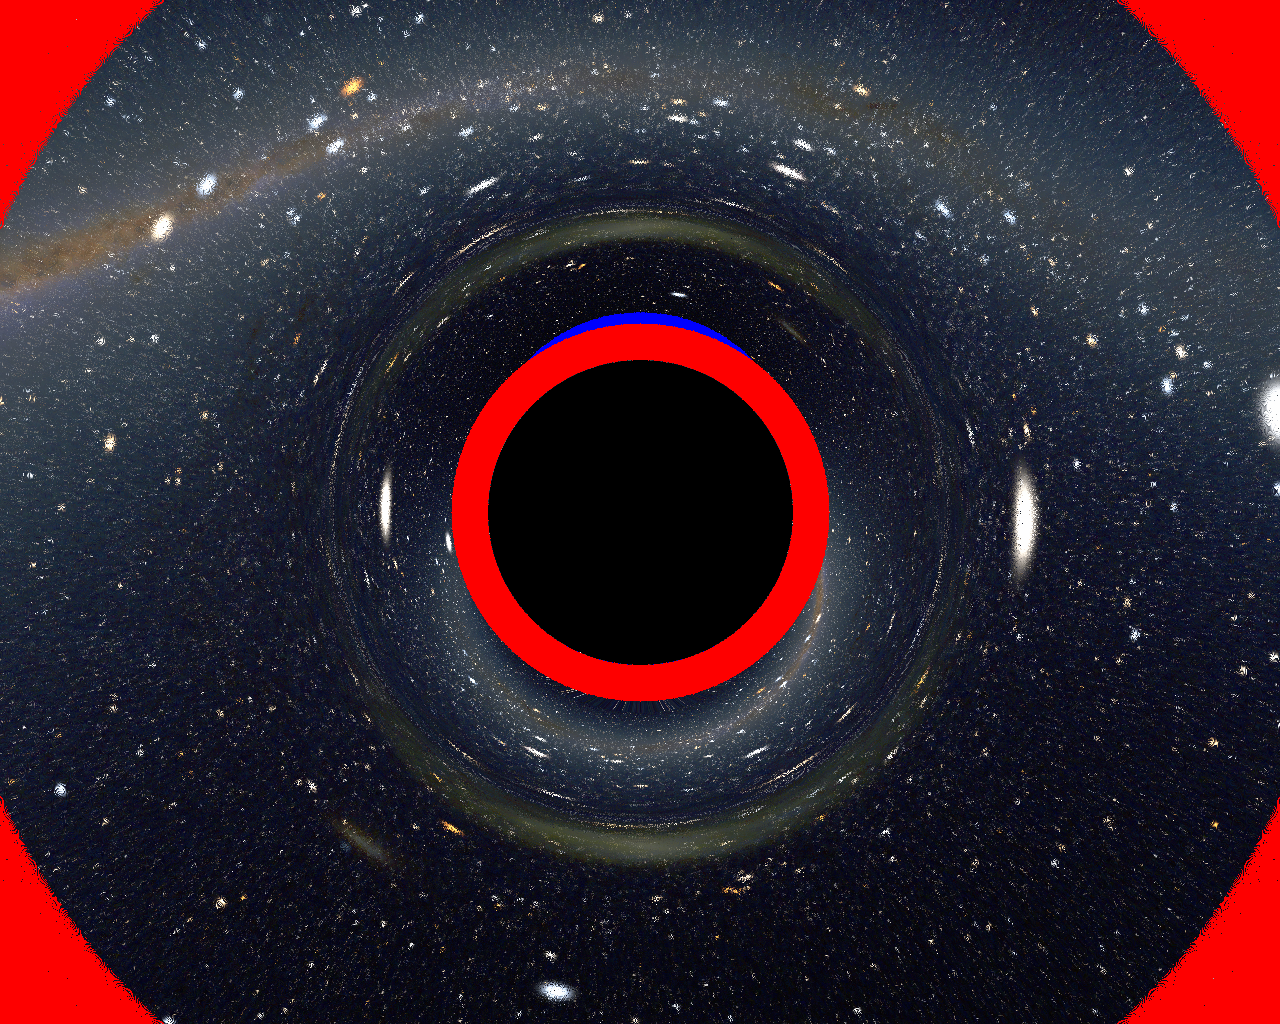
\includegraphics[width=.8\linewidth]{images/bhlens_erratum.png}
        \caption{使用Ray为单位进行追踪}
        \label{fig:nasa-apod-erratum}
    \end{subfigure}
\end{figure}



\section{离线渲染}
传统的光线追踪程序是通过判断光线(直线)与平面是否相交来判断是否光线是否击中物体的。近年随着消费级硬件性能提升,实时渲染领域光线追踪有取代光栅化的趋势。但也只是刚刚起步,只有最顶级的消费级显卡才能以Full HD画质在大多数游戏中实现令人满意的光线追踪渲染效果(60 FPS)。

黑洞附近的光线路径不再是直线,不能使用简单的直线求交方式判断光线的hit和miss。每一束光线都要多次迭代才能获得光束的起点。实时渲染并非不可行,却是以精度为代价的。我想专注于离线渲染达到较好的效果。
\subsection{World Space}
在本程序中世界坐标使用右手定则,上方为y轴正半轴,右方为x轴正半轴,后方为z轴正半轴。



\subsection{Camera Space}
每一个场景有一个观察者自身的Local Space也称Camera Space。观察者在Local Space的三个坐标在具有如下性质:Z负半轴为相机正前方,Y正半轴为相机正上方,X正半轴为相机右方。确定两个方向的世界坐标可以确定相机的位置和方向。

\subsubsection{相机坐标系到世界坐标系的转换}


相机拥有一个纵向视场(FoV)和一个横向视场,用于控制光线捕捉的最大张角。



\section{实时渲染}
\subsection{实现方式}
\subsection{时间复杂度}
\subsection{积分方法}
\subsection{积分近似}